\section{Złożenie projektu}
    Ostatnim krokiem, było napisanie, prostej gry w języku Python.
    Wybraną grą był Pong -- prosta gra w której gracz za pomocą wychylania akcelerometry jest w stanie sterować ruchami paletki.
    Głównym powodem wyboru tej gry było, to że reakcje gracza muszą być interpretowane w czasie rzeczywistym, a wszystkie spowolnienia będą bardzo widoczne.
    \begin{figure}[!ht]
        \centering
        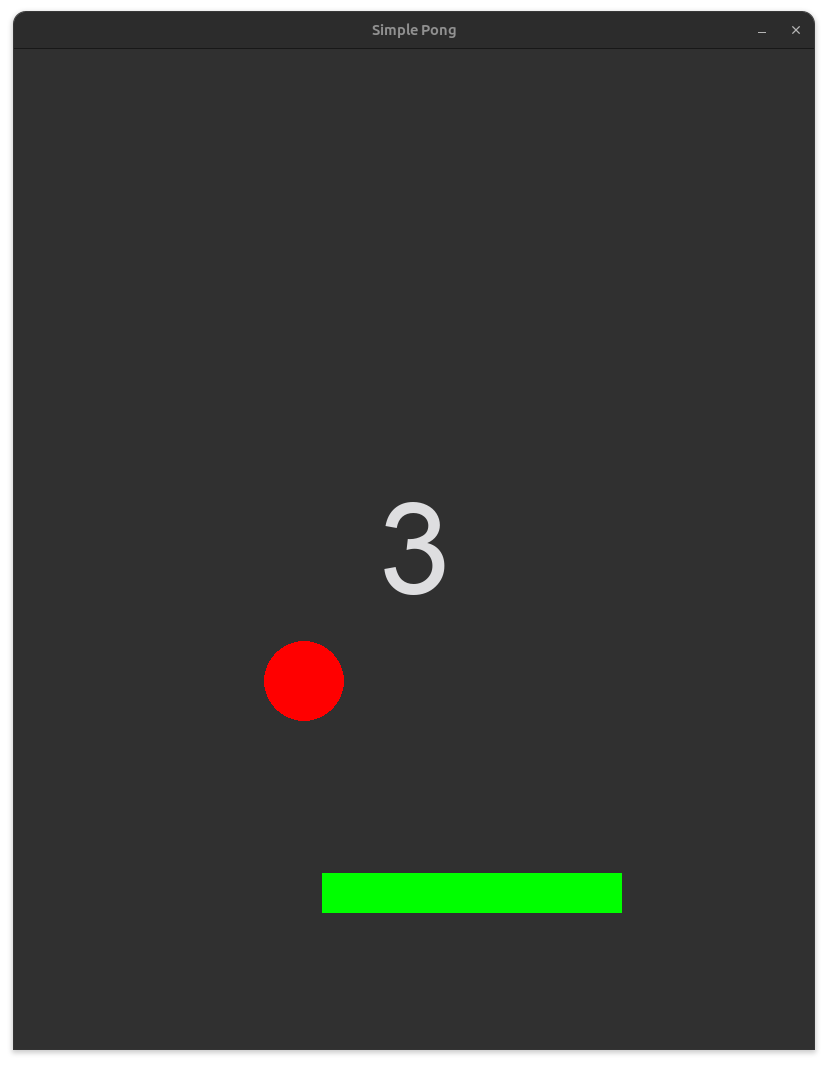
\includegraphics[width=0.4\textwidth]{pong.png}
        \caption{Gra Pong}
        \label{fig:pong}
    \end{figure}

    Rysunek \ref{fig:pong} przedstawia wyżej wymienioną grę z zaimplementowanym system sterowania ruchowego.

\section{Podsumowanie}
    Projekt zakończył się sukcesem, wszystkie założenia zostały spełnione.
    Jednak wykorzystanie standardu TCP do komunikacji w czasie rzeczywistym okazała się bardzo słabym wyborem.
    Aby układ pracował szybko oraz poprawnie, musiał został użyty jeden rdzeń na komunikację, zostawiający tylko jeden z dwóch dostępnych.
    Dodatkowo, okazyjnie zauważalne jest spowolnienie wynikające z tego że kontroler potrzebuje czasu aby odesłać odpowiedź do serwera.
    W mniej wymagającym czasowo scenariuszu, wykorzystane protokołu TCP może byś niezwykle użyteczne, a napisana biblioteka wykorzystana wielokrotnie.